% !TeX root = ../main.tex

\newlecture[Weak and Strong Law of Large Numbers]

\begin{theorem}[Basic WLLN][6.1]
    Let $X_1, X_2, \dots$ be independent. For all $i$, suppose $EX_i = \mu$ and $\Var(X_i) \leq \sigma^2 < \infty$. Define $S_n = \sum_{i=1}^n X_i$, then
    \[\bar{X}_n = \frac{1}{n}S_n \overset{P}{\longrightarrow} \mu\]
    \begin{proof}
        By linearity, we know
        \[E(\bar{X}_n) = \mu \quad \text{and} \quad \Var(\bar{X}_n) = \frac{\sigma^2}{n}\]
        By Chebyshev's inequality,
        \[\lim_{n\to\infty} P(|\bar{X}_n - \mu| \geq \varepsilon) \leq \lim_{n\to\infty}\frac{\sigma^2}{n\varepsilon^2} = 0\]
    \end{proof}
\end{theorem}

\begin{center}
\begin{tikzpicture}[scale=1, every node/.style={font=\small}]
    \draw[->] (0,-1.6) -- (0,1.8) node[above]{$\bar{X}_n$};
    \draw[->] (-0.2,0) -- (6,0) node[right]{$n$};
    \draw[dashed] (0,0.25) -- (5.8,0.25);
    \node[left] at (0,0.25) {$\mu$};
    \draw[dashed, gray] (0,1.5) .. controls (2,0.9) and (4,0.45) .. (5.8,0.35);
    \draw[dashed, gray] (0,-1.3) .. controls (2,-0.5) and (4,0.05) .. (5.8,0.15);
    \draw[thick, blue!55!black] plot[smooth, tension=0.7] coordinates {(0,0.6) (0.4,1.3) (1,-0.2) (1.6,-1.0) (2.3,0.8) (3,-0.1) (3.6,0.5) (4.3,0.15) (5,0.32) (5.8,0.25)};
    \node[red!70!black] at (4.6,1.4) {$\bar{X}_n \overset{P}{\longrightarrow} \mu$};
\end{tikzpicture}
\end{center}

\begin{theorem}[Uncorrelated WLLN][6.1.1]
    If $X_1, X_2, \dots$ are \underline{uncorrelated} with $EX_i = \mu$ and $\Var(X_i) \leq \sigma^2 < \infty$,
    \[\bar{X}_n \overset{P}{\longrightarrow} \mu\]
    (Replace ``independent'' by ``uncorrelated''.)
    \begin{proof}
        \[E(\bar{X}_n - \mu)^2 \to 0 \quad \Leftarrow \quad \bar{X}_n \ L^2 \text{ converge to } \mu\]
        \heading{Aside: $L^p$ converge}
        If $E[|X_n - \mu|^p] \to 0$, then we say $X_n$ $L^p$-converge to $\mu$.

        As $X_1, \dots, X_n, \dots$ have $E(X_i) = \mu$, $\Var(X_i) \leq \sigma^2 < \infty$ and are uncorrelated,
        \begin{align*}
            E[(\bar{X}_n - \mu)^2] &= \Var(\bar{X}_n)\\
            &= \frac{\sigma^2}{n}
        \end{align*}
        \[\lim_{n\to\infty} E[(\bar{X}_n - \mu)^2] = \lim_{n\to\infty}\frac{\sigma^2}{n} = 0\]
        So $\bar{X}_n$ $L^2$ converges to $\mu$. By Chebyshev's inequality,
        \[\bar{X}_n \overset{P}{\longrightarrow} \mu\]
        In fact,
        \[\underbrace{L^p \text{ converge}}_{\text{stronger}} \Rightarrow \underbrace{\text{converge in probability}}_{\text{weaker}} \quad \text{for any } p \in \N_+\]
    \end{proof}
\end{theorem}

\begin{exercise}[][\relax]
    Show that $L^2$ converge $\Rightarrow$ converge in $P$:
    \[E[(\bar{X}_n - \mu)^2] \to 0 \Rightarrow \bar{X}_n \overset{P}{\longrightarrow} \mu\]
\end{exercise}

\begin{theorem}[$L^1$ version WLLN][6.1.2]
    If $X_1, \dots, X_n$ are i.i.d.\ with $E|X_i| < \infty$ and $EX_i = \mu$, then
    \[\bar{X}_n \overset{P}{\longrightarrow} \mu\]
    (For this version, we dropped $\Var(X_i) = \sigma^2 < \infty$; we only require $E|X_i| < \infty$, and we have the same conclusion.)
    \\Proof is not required.
\end{theorem}

\begin{theorem}[Strong Law of Large Numbers][6.2]
    If $X_1, X_2, \dots$ are i.i.d.\ with $E|X_i| < \infty$ and $EX_i = \mu$, then
    \[\bar{X}_n = \frac{1}{n}\sum_{i=1}^n X_i \overset{a.s.}{\longrightarrow} \mu\]
    The SLLN is the strongest, in a way that it requires the \underline{fewest} conditions:
    \begin{enumerate}
        \item i.i.d.
        \item 1st moment exists, $E|X_i| < \infty$
    \end{enumerate}
    but provides the strongest conclusion $\bar{X}_n \overset{a.s.}{\longrightarrow} \mu$.
    \\(Proof is beyond the scope of this course.)
\end{theorem}

\heading{Summary Table of LLN}
\begin{center}
\small
\begin{tabular}{l|cccc}
    & Requirement 1 & Requirement 2 & Requirement 3 & Conclusion\\
    & independence & identical & $\Var(X_i) < \infty$ & $\overset{P}{\to}$ / $\overset{a.s.}{\to}$\\
    \hline
    {\color{blue!55!black}WLLN} & {\color{blue!55!black}\shortstack{uncorrelated\\ always OK}} & {\color{blue!55!black}always drop} & {\color{blue!55!black}always drop} & {\color{blue!55!black}$\overset{P}{\to}$ \checkmark}\\
    {\color{red!70!black}SLLN} & {\color{red!70!black}need} & {\color{red!70!black}drop} & {\color{red!70!black}drop} & {\color{red!70!black}$\overset{a.s.}{\to}$ \checkmark}
\end{tabular}
\end{center}

\begin{theorem}[A weaker version of SLLN][6.2.1]
    Let $X_1, X_2, \dots$ be independent, and for all $i$, suppose $E(X_i) = \mu$ and $E(X_i - \mu)^4 \leq a < \infty$. Then,
    \[\bar{X}_n = \frac{1}{n}\sum_{i=1}^n X_i \overset{a.s.}{\longrightarrow} \mu\]
    (The 4th moment condition is only required for proving the SLLN in this course!)
    \begin{proof}
        Without loss of generality, we assume $\mu = 0$.
        \begin{align*}
            ES_n^4 &= E\left[\left(\sum_{i=1}^n X_i\right)^4\right]\\
            &= E\Big(\sum_{i=1}^n X_i^4 + \underbrace{k_1\sum_{i=1}^n\sum_{j\neq i} X_i^3X_j}_{E(\cdot) = 0} + k_2\sum_{i=1}^n\sum_{j\neq i} X_i^2X_j^2\\
            &\qquad + \underbrace{k_3\sum_{i=1}^n\sum_{j\neq i}\sum_{k\neq i,j} X_i^2X_jX_k}_{E(\cdot) = 0} + \underbrace{k_4\sum_{i=1}^n\sum_{j\neq i}\sum_{k\neq i,j}\sum_{l\neq i,j,k} X_iX_jX_kX_l}_{E(\cdot) = 0}\Big)
        \end{align*}
        The cross terms vanish by independence, e.g.
        \[E\Big[k_1\sum\sum X_i^3X_j\Big] = k_1\sum\sum E(X_i^3)\underbrace{E(X_j)}_{=0} = 0\]
        \[E\Big[k_3\sum\sum\sum X_i^2X_jX_k\Big] = k_3\sum\sum\sum E(X_i^2)\underbrace{E(X_j)}_{=0}\underbrace{E(X_k)}_{=0} = 0\]
        So
        \begin{align*}
            ES_n^4 &= E\left(\sum_{i=1}^n X_i^4\right) + E\left(k_2\sum_{i=1}^n\sum_{j\neq i} X_i^2X_j^2\right)\\
            &= \sum_{i=1}^n \underbrace{E(X_i^4)}_{\leq a} + k_2\sum_{i=1}^n\sum_{j\neq i}\underbrace{E(X_i^2)}_{\leq b}\underbrace{E(X_j^2)}_{\leq b}
        \end{align*}
        since $E(X_i^4) \leq a$ and $E(X_i^2) \leq b$ for some $a$ and $b$.
        \begin{align*}
            &\leq na + k_2 n(n-1)b^2\\
            &\leq Kn^2 \qquad \text{for some constant } K
        \end{align*}
        For any $\varepsilon > 0$, apply Markov's inequality ($P(X > a) \leq \frac{E(X)}{a}$):
        \begin{align*}
            P(|\bar{X}_n| > \varepsilon) &= P(S_n^4 > n^4\varepsilon^4)\\
            &\leq \frac{ES_n^4}{n^4\varepsilon^4}\\
            &\leq \frac{Kn^2}{n^4\varepsilon^4} & &\text{we showed that } ES_n^4 \leq Kn^2\\
            &= \frac{K}{n^2\varepsilon^4} = C\cdot\frac{1}{n^2}
        \end{align*}
        \[\sum_{n=1}^\infty C\cdot\frac{1}{n^2} < \infty \qquad \text{(the sequence $\tfrac{1}{n^2}$ has finite sum)}\]
        \begin{center}
            \fbox{$\displaystyle\sum_{n=1}^\infty \frac{1}{n} = \infty, \qquad \sum_{n=1}^\infty \frac{1}{n^2} < \infty$}
        \end{center}
        By the Borel-Cantelli Lemma (Prop 5.5.2),
        \[\Rightarrow \bar{X}_n \overset{a.s.}{\longrightarrow} \mu\]
    \end{proof}
\end{theorem}
